\documentclass[11pt,reqno]{amsart}
\usepackage{amsmath,amsthm,amsfonts, amssymb}
\usepackage{mathptmx}
\usepackage{mathtools} %\xleftarrow[]{}
% \usepackage{mathrsfs}
% \usepackage[all]{xy}
% \usepackage{stmaryrd}
% \usepackage{fancyhdr}

\usepackage{pgf, tikz}
\usetikzlibrary{arrows, automata}

\usepackage{tikz-cd}
% \usepackage{cite}
% \usepackage{amsmath, amsfonts}
\usepackage{graphicx}
\usepackage{wrapfig}
% \usepackage{array}
% \usepackage{exercise}
\usepackage{hyperref}
\usepackage{cleveref} % Add for \Cref, \cref

% \usepackage{enumerate}
\usepackage[shortlabels]{enumitem}
% \usepackage{tikz}

\pagestyle{plain}
\usepackage[left=1.2in, right=1.2in, top=1in, bottom=1in]{geometry}
\usepackage{etoolbox}
% \usepackage{color}
\usepackage{xcolor}
\patchcmd{\section}{\scshape}{\bfseries}{}{}
\makeatletter
\renewcommand{\@secnumfont}{\bfseries}
\makeatother
% \xyoption{all}
\thispagestyle{empty}

\DeclareMathOperator{\Hom}{Hom}
\DeclareMathOperator{\Spec}{Spec}
\DeclareMathOperator{\Frac}{Frac}
\DeclareMathOperator{\Img}{Img}
\DeclareMathOperator{\Ker}{Ker}
\DeclareMathOperator{\Pic}{Pic}
\DeclareMathOperator{\Jac}{Jac}
\DeclareMathOperator{\Div}{Div}
\DeclareMathOperator{\dv}{Div}
\DeclareMathOperator{\Deg}{deg}
\DeclareMathOperator{\Aut}{Aut}
\DeclareMathOperator{\snf}{SNF}

\newcommand\scalemath[2]{\scalebox{#1}{\mbox{\ensuremath{\displaystyle #2}}}}
\newcommand{\angles}[1]{\langle #1 \rangle}
\newcommand{\R}{\mathbb{R}}  
\newcommand{\Z}{\mathbb{Z}}
\newcommand{\N}{\mathbb{N}}
\newcommand{\Q}{\mathbb{Q}}
\newcommand{\I}{\mathbf{I}}

\newcommand{\jaiung}[1]{{\textcolor{red}{Jaiung: #1}}}
\newcommand{\youngsu}[1]{{\textcolor{blue}{Youngsu: #1}}}
\newcommand{\matt}[1]{{\textcolor{cyon}{Matt: #1}}}

% \input xy
% \xyoption{all}
\thispagestyle{empty}

%\usepackage{secdot}

\theoremstyle{definition}
\newtheorem{mydef}{Definition}[section]
\newtheorem{myeg}[mydef]{Example}
\newtheorem{conj}[mydef]{Conjecture}
\newtheorem*{noconj}{Conjecture}
\newtheorem{observ}[mydef]{Observation}
\newtheorem{question}[mydef]{Question}
\newtheorem{rmk}[mydef]{Remark}
\newtheorem*{que}{Question}
\newtheorem*{goal}{Goal}

\theoremstyle{plain}
\newtheorem{mythm}[mydef]{Theorem}
\newtheorem*{nothm}{Theorem}
\newtheorem*{nomainthm}{Main Theorem}
\newtheorem*{nothma}{Theorem A}
 \newtheorem*{nothmb}{Theorem B}
 \newtheorem*{nothmc}{Theorem C}
% \newtheorem*{nothmd}{Theorem D}
% \newtheorem*{nothme}{Theorem E}
% \newtheorem*{nothmf}{Theorem F}
% \newtheorem*{nothmg}{Theorem G}
\newtheorem{mytheorem}[mydef]{Theorem}
\newtheorem{lem}[mydef]{Lemma}
\newtheorem{lemma}[mydef]{Lemma}
\newtheorem{pro}[mydef]{Proposition}
\newtheorem{proposition}[mydef]{Proposition}
\newtheorem{claim}[mydef]{Claim}
\newtheorem{cor}[mydef]{Corollary}
\newtheorem{con}[mydef]{Construction}

% \patchcmd{\abstract}{\scshape\abstractname}{\normalsize{\textbf{\abstractname}}}{}{}
\begin{document}

\title{On Picard groups of directed graphs}

\author{Jaiung Jun}
\address{Department of Mathematics, State University of New York at New Paltz, NY 12561, USA}
\email{junj@newpaltz.edu}

\author{Youngsu Kim}
\address{Department of Mathematics, California State University San Bernardino, San Bernardino, CA 92407}
% \curraddr{}
\email{youngsu.kim@csusb.edu}

\author{Matthew Pisano}
\address{Department of Computer Science, State University of New York at New Paltz, NY 12561, USA}
\email{pisanom1@newpaltz.edu}

\makeatletter
\@namedef{subjclassname@2020}{
	\textup{2020} Mathematics Subject Classification}
\makeatother

\subjclass[2020]{05C50, 05C76}
\keywords{Jacobian of a graph, sandpile group, critical group, chip-firing game, directed graphs, cycle graph, wheel graphs, Laplacian of graph, trees, Smith normal form}

\maketitle

\begin{abstract}
The Picard group $\Pic(G)$ of a graph $G$ is a finitely generated abelian group, and the Jacobian $\Jac(G)$ is the torsion subgroup of $\Pic(G)$. These groups can be computed by using the Smith normal from of the Laplacian matrix $L_G$ or by using chip-firing games. One may consider its generalization to directed graphs by using Laplacian matrices. In this paper, we investigate Picard groups and Jacobians for several classes of directed graphs, including directed trees and directed cycles. Different from the undirected case, even for trees and cycles, one can find very interesting computational results. Our investigation is based on experimental mathematics; we compute a large number of examples, find some patterns from them, and prove them. 
\end{abstract}

\section{Introduction}

%%%%%%%%%%%%%%%%%%%%%%%%%%%%% bacgrkound %%%%%%%%%%%%%%%%%%%%%%%%%%%


A chip-firing game is a combinatorial game that one can play on finite graphs. To play a chip-firing game, one first puts chips (possibly negative as ``debt'') at each vertex of a graph $G$. At each turn, a vertex can borrow / lend chips from / to all neighbors simultaneously. The goal of the game is to find a finite sequence of borrowing / lending moves so that every vertex is debt-free. Hence, a natural question to ask is whether or not one can determine there is a winning moves for a given configuration of chips. 

To study the game more systemically, one can write any chip configuration as an element of the free abelian group generated by the set of vertices $V(G)$ of a graph $G$ which is denoted by $\Div(G)$. Each element of $\Div(G)$ is called a divisor, and a divisor $D$ is effective if $D=\sum_{v \in V(G)} a_vv$, with $a_v \geq 0$. Then, one defines an equivalence relation on $\Div(G)$ as follows: $D\sim D'$ if and only if $D'$ can be obtained from $D$ by a finite sequence of borrowing / lending movers. This defines a group 
\[
\Pic(G):=\Div(G)/\sim,
\]
called the Picard group of $G$. The torsion subgroup of $\Pic(G)$, denoted by $\Jac(G)$, is called the Jacobian of $G$.\footnote{Depending on literature, $\Jac(G)$ is also called as a critical group.}

The combinatorial theory of chip-firing games has connections to various areas in mathematics. For instance, from a perspective motivated by algebraic geometry, one may view finite graphs as a discrete model for Riemann surfaces. In this case, chip configurations play the role of divisors on curves. In fact, Baker and Norine \cite{baker2007riemann} formulated and proved a version of Riemann-Roch theorem for finite graphs as follows:
\[
r(D) - r(K-D) = \deg(D) -g+1,
\]
where $g=|E(G)|-|V(G)|+1$, $\deg(D)$ for $D \Pic(G)$ is the total number of chips, $K=\sum_{v \in V(G)} (\deg(v)-2)v \in \Div(G)$ (the canonical divisor of $G$), and the rank $r(D)$ is one less than the minimum number of chips which need to be removed so that $D$ is no longer equivalent to an effective divisor. When $G$ is a dual graph of a strongly semistable model for an algebraic curve $X$ (smooth, proper, geometrically connected) over a valued field, one also has a (degree-preserving) group homomorphism $\rho:\Pic(X) \to \Pic(G)$. 

For a graph $G$ with the vertices $\{v_1,v_2,\dots,v_n\}$, one defines an $n\times n$ matrix $L_G$, called the Laplacian matrix of $G$, as follows:
\[
(L_G)_{ij}=\begin{cases}
\textrm{ valency of $v_i$}, \quad i=j\\
-(\textrm{\# of edges between $v_j$ and $v_j$}), \quad i \neq j.
\end{cases}
\]
To compute $\Pic(G)$, one can use the Laplacian matrix $L_G$ of a graph $G$. One can easily check that any configuration of chips can be considered as a vector $v \in \mathbb{Z}^{V(G)}$, and the chip configuration $v'$ by making a lending move (resp.~borrowing move) at a vertex $i$ from $v$ is the following:
\begin{equation}\label{eq: introduc1}
v'=v - (L_G^t)e_i \quad (\textrm{resp.~} v'=v + (L_G^t)e_i).
\end{equation}
With this, by considering $L_G^t:\mathbb{Z}^{V(G)} \to \mathbb{Z}^{V(G)}$, one can see that $\Pic(G)=\textrm{coker}(L_G^t)$, and $\Pic(G)=\mathbb{Z}\times \Jac(G)$. 



From \eqref{eq: introduc1}, one is naturally led to think that one can play a chip-firing game with a given matrix $M$ (replacing $L_G$), namely firing at a site $i$ is:
\begin{equation}\label{eq: introduc2}
	v'=v - (M^t)e_i.
\end{equation}


Now we specialize the case when a matrix $A$ is a directed Laplacian. Perhaps we need to cite some results in Section 6 of \cite{klivans2018mathematics}


%%%%%%%%%%%%%%%%%%%%%%%%%%%%%%%%%%%%%%%%%%%%%%%%%%%%%%%%%%%%%%%%%%%%


%%%%%%%%%%%%%%%%%%%%%%%% put our results in context below %%%%%%%%%%%%%%%%%%%%%%%%

\subsection{to be edited}



The main things that we have done so far:
\begin{enumerate}
	\item 
$\Jac(T)=\{0\}$ (Proposition \ref{proposition: tree proposition}). 
\item 
$\Jac(C_n)$ can be anything (Conjecture \ref{conjecture: single term}). 
\item 
An explicit construction of an orientation of $C_n$ so that $\Jac(C_n)=\mathbb{Z}_m$ (Conjecture \ref{conjecture: two path}). 
\end{enumerate}

The remaining things that we want to do:
\begin{enumerate}
	\item 
Add experimental data visualization for number of paths needed and sizes of graphs. 
	\item 
Anything else??
\end{enumerate}

Things that we might want to do (or perhaps leave them as conjectures):
\begin{enumerate}
	\item 
Proof of wheel graph conjecture (should be rewritten with Lucas numbers). \cite{biggs1999chip} should be relevant. 
\item 
Proof of multipartite graphs. \cite{jacobson2003critical} could be relevant. 
\end{enumerate}

\begin{nothma}
Let $T$ be a tree with any orientation. Then $\Jac(T)=\{0\}$. 
\end{nothma}

\begin{nothmb}
Let $C_n$ be a cycle graph with $n$ vertices. For any $0 \leq m \leq n$, there exists an orientation of $C_n$ such that $\Jac(C_n)=\mathbb{Z}_m$ with the orientation. Furthermore, we explicitly describe how to find an orientation of $C_n$ to obtain $\mathbb{Z}_m$. 
\end{nothmb}

For all bidirectional edges, Biggs computed the Jacobian of a wheel graph in \cite{biggs1999chip}. For the directional cases, we compute two special cases. Let $W_n$ be the wheel graph on $n$-vertices with bidirectional edges, and $W_n'$ with the edges of the rim are bidirecional and all its spoke edges point to the axel. Let $W_n{''}$ be the wheel graph on $n$-vertices where the edges of the rim are bidirecional and all its spoke edges point away from the axel. 

\begin{nothmc}
With the same notation as above, we have the following. 
\begin{enumerate}
	\item 
The Lapacian matrices of $W_n$ and $W_n'$ are row equivalent. In particuar, one has $\Pic (W_n) \cong \Pic (W_n')$.	
	\item 
The smith normal form of the Laplician of $W_n^{''}$ is of the form 
\begin{equation*}
	\left[
	\begin{array}{c|ccc}	
		I_{n-3} & 0 & 0 & 0 \\
		\hline
		0 & a & 0 & 0 \\
		0 & 0 & b & 0 \\
		0 & 0 & 0 & 0 
	\end{array}
	\right],
\end{equation*}
where 
$(a,b) = \begin{cases}
	(n-1,n-1) & \text{if}~ n ~\text{is even}; \\
	(\frac{n-1}2, 2(n-1)) & \text{if}~ n ~\text{is odd}
\end{cases}$.	
\end{enumerate}
\end{nothmc}

%%%%%%%%%%%%%%%%%%%%%%%%%%%%%%%%%%%%%%%%%%%%%%%%%%%%%%%%%%%%%%%%%%%%%%%%%%%%%%%%


%\begin{goal}[8/1/2022]$ $
%	\begin{enumerate}
%		\item
%		Prove/disprove: for an oriented graph $G$, one always has $\Pic(G)=\mathbb{Z} \times \Jac(G)$,
%		i.e., as a finitely generated abelian group, the rank of $\Pic(G)$ is $1$.
%		\textcolor{red}{Jaiung: we disproved this by using~\cite{wagner2000critical}.}
%		\item
%		Prove/disprove: for $C_n$, and $0 \leq m \leq n$, one can always find an orientation
%		of $C_n$ so that $\Jac(C_n)=\mathbb{Z}_m$ (with the orientation).
%		\item
%		Prove/disprove: for an oriented graph $G$, if $v_0 \in V(G)$ is a sink (or a source)
%		and $G'$ is the graph obtained by reserving the direction for all arrows adjacent
%		to $v_0$ from $G$, then $\Jac(G)=\Jac(G')$. (Note: we believe that this should be true
%		for at least some classes of graphs such as cyclic graphs.)
%		\item
%		Prove/disprove: for an oriented planar graph $G$ and its planar dual (should be defined)
%		$\hat{G}$, one has $\Jac(G)=\Jac(\hat{G})$.
%		\item
%		Prove/disprove: for oriented graphs $G_1,G_2$, let $G$ be the graph obtained by
%		gluing $G_1$ and $G_2$ along one vertex. Then $\Jac(G)=\Jac(G_1) \times \Jac(G_2)$.
%		\textcolor{red}{Jaiung: we are currently working on this (8/31)}
%	\end{enumerate}
%\end{goal}

	%This project will study Chip-Firing games and how different combinations of directed and undirected edges affect its winning strategies. We will focus on Research Project 11 in~\cite{glass2020chip}. Our plan is to pursue this for trees, cycle graphs, pseudotrees, and wheel graphs.

	% \youngsu{test}

		%We explore a combinatorial game on finite graphs, called Chip-Firing Games, which has various connections to other areas, such as algebraic geometry, number theory and economics. To play the game, one first puts an integer amount of chips at each vertex.  Then, each vertex is allowed to borrow or lend chips from its neighbors equally as the game progresses.One can study chip-firing games on a graph $G$ through a finitely generated abelian group	$\Pic(G)$ (Picard group) and its torsion subgroup $\Jac (G)$ (Jacobian) which canbe computed by using the Laplacian matrix of $G$.

	%When a graph $G$ is directed, one may extend the definition of $\Pic(G)$ and $\Jac (G)$ for undirected graphs by using Laplacian matrices.  However, computations become much more complicated. For example, $\Pic(G)=\mathbb{Z}$ for any undirected tree $G$. 	This follows from the matrix-tree theorem, which tells us that $|\Jac (G)|$ is	the number of spanning trees of an undirected graph $G$.In the case of directed trees, even the rank of $\Pic(T)$ can be arbitrarily large.Particularly, for any natural number $n$, we can construct a tree $T_n$ (a tree with $n$ vertices) such that the rank of $\Pic(T_n)$ is $n$.

	%In our ongoing project, we study Picard groups and Jacobians for directed trees, cycles, and pseudotrees.Even in these seemingly simple cases, we find some new phenomenon. For instance, for the undirected cycle $C_n$,$\Jac (C_n)=\mathbb{Z}_n$, however, we prove that in the directed case, for any given $0 \le m \leq n$, one can always find an orientation of $C_n$ in such a way that $\Jac (C_n)$ is $\mathbb{Z}_m$.	By closely examining trees and cycles, and how Picard groups and Jacobians change with (suitably defined)	vertex and edge gluing, we obtain several results for pseudotrees.

\bigskip


\textbf{Acknowledgment}\hspace{0.1cm} This research was supported by Research and Creative Activities (RSCA) at SUNY New Paltz. We would like to thank RSCA for their support. \textcolor{red}{Add here thanks to CSUSB HPC.}

\section{Preliminaries}

\begin{mydef}
	\textcolor{red}{Jaiung: Recall terminal strong components}
\end{mydef}

\begin{mytheorem}
\textcolor{red}{Jaiung: Here we recall \cite{wagner2000critical} the torsion-free part theorem. }
\end{mytheorem}

		\begin{rmk}\label{remark: embedding}
	Let $M \in M_{m \times n}(\mathbb{Z})$, 
	and let $I_k(M)$ denote the ideal generated by $k \times k$ minors of $M$, 
	where $I_k(M) = 0$ if $k > \min\{m,n\}$ and $I_k = (1)$ if $k \le 0$. 
	For a matrix $N = \left[ \begin{array}{c|c}
		M & 0 \\
		\hline
		0 & 1
	\end{array} \right]$ and for any $k$, $I_k(M) = I_{k+1}(N)$, and the cokernels of $M$ and $N$ are isomorphic. 
\end{rmk}

The following is well-known. For instance, wee \cite[Theorem 2.4]{stanley2016smith}.

\begin{mytheorem}\label{theorem: gcd theorem}
Let $R$ be a unique factorization domain such that any two elements have a greatest common divisor (gcd). Suppose that $M \in \emph{Mat}_{m \times n}(R)$ has a Smith normal form $L=(x_1,\dots,x_m)$. Then, for $1\leq k \leq m$, the product $x_1\cdot \cdots x_k$ is equal to the gcd of all $k\times k$ minors of $M$, with the convention that if all $k\times k$ minors are $0$ then their gcd is $0$. 
\end{mytheorem}

	%\subsection{Chip Firing}
	%	The game at the heart of this paper is the Chip-Firing game. When a game is started, each vertex on a graph is assigned a certain number of chips.  During play, chips can be lent or borrowed at each node where one or more chips are either sent or received along each outgoing edge equally.  In the case of a directed graph, vertices can only interact with another along an outgoing or bidirectional edge.  The game is won once every vertex has a positive number of chips (i.e., this vertex is not in debt).

%\subsection{Divisors and Equivalence Relations}
%		In the study of this game a \textbf{Divisor} of a graph ($\Div(G)$) is an integer vector $v\in\mathbb{Z}^n$ where \textit{n} is the number of vertices in the graph.  The $i^{th}$ element of the vector \textit{v} is the number of chips on the $i^{th}$ vertex of the graph.  Two divisors have an \textbf{equivalence relation} ($\sim$) if one divisor can be gotten from the other by a finite series of lending or borrowing moves $D_1 \sim D_2 \xleftrightarrow{} (D_1 \xleftrightarrow{\text{moves}} D_2)$.  For a divisor $D$, the \textbf{equivalence class} {$[D]$} is the set of all divisors that are equivalent to each other, $[D] = \{D_i~|~D_i \sim D\}$.

	%\subsection{The Picard Group and The Jacobian}
	%	The \textbf{Picard Group} of a graph $\Pic(G)$ is the set of all equivalence classes that the divisors of that graph can be a  part of. The \textbf{Jacobian} of a graph  $\Jac(G)$ is a subset of $\Pic(G)$ such that every divisor in each equivalence class has a degree of $0$, where the degree of a divisor $\Deg(D)$ is the sum of each of the divisor's elements. If a divisor is in one of the Jacobian's classes, it can be made winning after a finite series of moves. Here, we represent the Picard Group as $\Pic(G)=\Jac(G)\times\mathbb{Z}^n$.


\section{Picard groups of oriented trees}

\begin{lem}\label{proposition: gluing an arrow proposition}
Let $G$ be a directed graph. If we attach either an incoming arrow or a two-sided arrow to create another directed graph $G'$, then $\Pic(G)=\Pic(G')$.
\end{lem}
\begin{proof}
Let $\alpha$ be an arrow which is glued to $G$. Let $|V(G)|=n$. We label the vertexes of $G$ as $1,2,\dots,n$. Suppose first that $\alpha$ is incoming and $\alpha$ is glued at the vertex $n$. Let $L_G=(a_{ij})$ (resp.~$L_{G'}$) be the Laplacian matrix of $G$ (resp.~$G'$). 
Then the matrix $L_{G'}$ is of the following form.
% In this case, one can easily observe that the matrix $L_{G'}$ is of the following form:
\begin{equation}
L_{G'}=\left[\begin{array}{ccc|c|c}
a_{11}&a_{12}&\cdots &a_{1n}&0\\
a_{21}&a_{22}&\cdots &a_{2n}&0\\
\vdots & \vdots &\ddots & \vdots & \vdots \\ \hline
\vdots & \vdots & \cdots&a_n & 0\\ \hline
0&0&\cdots &-1&1\\
\end{array}\right]
\end{equation}
		By a column operation between the last two columns, we obtain the following matrix:
		\begin{equation}\label{eq: arrow adding matrix}
			\left[\begin{array}{ccc|c|c}
				a_{11}&a_{12}&\cdots &a_{1n}&0\\
				a_{21}&a_{22}&\cdots &a_{2n}&0\\
				\vdots & \vdots &\ddots & \vdots & \vdots \\ \hline
				\vdots & \vdots & \cdots&a_n & 0\\ \hline
				0&0&\cdots &0&1\\
			\end{array}\right]
		\end{equation}
		This shows that $\Pic(G)=\Pic(G')$.

		Next, suppose that $\alpha$ is a two-sided arrow. Then similar to the above, we obtain the following Laplacian matrix for $G'$:
		\begin{equation}\label{eq: eq two-sided}
			L_{G'}=\left[\begin{array}{ccc|c|c}
				a_{11}&a_{12}&\cdots &a_{1n}&0\\
				a_{21}&a_{22}&\cdots &a_{2n}&0\\
				\vdots & \vdots &\ddots & \vdots & \vdots \\ \hline
				\vdots & \vdots & \cdots&a_n+1 & -1\\ \hline
				0&0&\cdots &-1&1\\
			\end{array}\right]
		\end{equation}
		By a column operation, the matrix~\eqref{eq: eq two-sided} becomes the matrix~\eqref{eq: arrow adding matrix}.
		This shows that $\Pic(G)=\Pic(G')$.
	\end{proof}



%\begin{conj}
%	The Jacobian of a tree graph is always trivial.  It follows from the matrix-tree theorem as a tree graph only has one possible spanning tree. \textcolor{red}{[Citation Needed]} \end{conj}

The following example shows that if we change the direction of arrows, Picard groups can change drastically.

\begin{myeg}\label{example: tree four}
Consider the following directed tree:
\begin{equation}\label{eq: tree4}
T=\left(\begin{tikzcd}
	& 1 \arrow[d] & \\
2 \arrow[r]& 3 & 4 \arrow[l]\\
& 5 \arrow[u] &
\end{tikzcd} \right)
\end{equation}
We have
\[
L_T = \begin{bmatrix}
 1& 0& -1&0 &0 \\
 0 & 1 & -1 & 0 &0\\
 0& 0& 0& 0 &0\\
 0& 0&-1&1 & 0\\
 0& 0&-1&0 & 1
\end{bmatrix} \implies \snf(L_T)=\left[\begin{array}{c|c}
I_4 & 0 \\ \hline
0 & 0
\end{array}\right]
\]
Hence, $\Pic(T)=\mathbb{Z}$. On the other hand, consider the following
\begin{equation}
T'=\left(\begin{tikzcd}
		& 1 & \\
		2 & 3 \arrow[u] \arrow[r]\arrow[l] \arrow[d]& 4 \\
		& 5  &
	\end{tikzcd} \right)
\end{equation}
We have
\[
L_T = \begin{bmatrix}
	0& 0& 0&0 &0 \\
	0 & 0 & 0 & 0 &0\\
	1& 1& 4& 1 &1\\
	0& 0&0&0 & 0\\
	0& 0&0&0 & 0
\end{bmatrix} \implies \Pic(T')=\mathbb{Z}^4.
\]
\end{myeg}

\begin{rmk}
For the undirected case, when one glues two graphs $G_1$ and $G_2$ along one vertex to obtain $G$, then $\Pic(G)=\Pic(G_1) \times \Pic(G_2)$. But, this is no longer true for directed graphs. For instance, the tree $T$ in \eqref{eq: tree4} can be considered as a directed graph obtained by gluing the following two directed graphs $G_1$ and $G_2$ along the vertices $3$ and $3'$"
\begin{equation}
G_1=\left(\begin{tikzcd}
	& 1 \arrow[d] & \\
	2 \arrow[r]& 3 
\end{tikzcd} \right), \quad G_2=\left(\begin{tikzcd}
& 3' & 4 \arrow[l]\\
& 5 \arrow[u] &
\end{tikzcd} \right)
\end{equation}
But, we have
\[
L_{G_1}=\begin{bmatrix}
	1 & 0 &-1\\
	0 & 1 & -1\\
	0& 0 & 0
\end{bmatrix} \implies \Pic(G_1)=\mathbb{Z}, \quad L_{G_2}=\begin{bmatrix}
0 & 0 &0\\
-1 & 1 & 0\\
-1& 0 & 1
\end{bmatrix} \implies \Pic(G_2)=\mathbb{Z}
\]
It follows that $\Pic(T) \neq \Pic(G_1) \times \Pic(G_2)$.
\end{rmk}

For the undirected trees $T$, $\Pic(T)=\mathbb{Z}$. But, for directed trees, the rank of $\Pic(T)$ can be arbitrarily large depending the number of strong terminal component of $T$. Nonetheless, we prove that $\Jac(T)=\{0\}$ in the following. 

\begin{pro}\label{proposition: tree proposition}
Let $T$ be a tree with any orientation. Then $\Jac(T)=\{0\}$, i.e., $\Pic(T)$ is torsion-free.
\end{pro}
\begin{proof}
We inductively prove this. When $T_0$ is a tree with one arrow, one can easily check that $\Pic(T_0) =\mathbb{Z}$ or $\{0\}$ (depending on the number of strong terminal components).

Suppose that $T_k$ is an oriented tree with $k$ arrows. When we add one arrow $\alpha$ to $T_k$ to construct $T_{k+1}$, there are three cases; $\alpha$ is $(1)$ incoming, $(2)$ outgoing, and $(3)$ two-sided. When $\alpha$ is either incoming or two-sided arrow, then it follows from Lemma \ref{proposition: gluing an arrow proposition} that $\Pic(T_k)=\Pic(T_{k+1})=\mathbb{Z}^r$, where $r$ is the number of the terminal strong components of $T_k$ and $T_{k+1}$, since in this case it does not increase the number of the terminal strong components.

Next, suppose that $\alpha$ is an outgoing arrow. Let's label the vertexes of $G$ as $v_1,v_2,\dots,v_n$. Suppose that the arrow $\alpha$ is attached to the vertex $v_j$. Let $L_{k}=(a_{ij})$ be the Laplacian matrix of $T_k$. Then we have the following:
\begin{equation}\label{eq: tree case}
L_{{k+1}}=\left[\begin{array}{ccccc|c|c}
a_{11}&a_{12}&\cdots& a_{1j}& \cdots&a_{1n}&0\\
a_{21}&a_{22}&\cdots& a_{2j}& \cdots&a_{2n}&0\\
\vdots & \vdots &\ddots&\vdots & \vdots&\vdots & \vdots \\
a_{j1}&a_{j2}&\cdots& a_{jj}+1 & \cdots&a_{jn}&-1\\
\vdots & \vdots & \cdots&\vdots &\vdots &\vdots & \vdots\\
a_{n1}&a_{n2}&\cdots& a_{nj} & \cdots&a_{nn}& 0\\  \hline
0&0&\cdots&\cdots &0 &0&0\\
\end{array}\right]
\end{equation}
To compute the Smith normal form, by relabeling vertices, we may assume $L_{k+1}$ is the following matrix:
\begin{equation}\label{eq: tree case2}
\left[\begin{array}{ccc|c|c}
		a_{11}&a_{12}&\cdots &a_{1n}&0\\
		a_{21}&a_{22}&\cdots &a_{2n}&0\\
		\vdots & \vdots &\ddots & \vdots & \vdots \\ \hline
		\vdots & \vdots & \cdots&a_n & 1\\ \hline
		0&0&\cdots &0&0\\
	\end{array}\right]
\end{equation}
Since $\Pic(T_k)=\mathbb{Z}^r$, there exist $P, Q \in \textrm{GL}_n(\mathbb{Z})$ such that
\begin{equation}
PL_kQ = \left[\begin{array}{c|c}
			I_{n-r} & 0 \\ \hline
	0 & 0_r
\end{array}\right]
\end{equation}
where $0_r$ is an $r\times r$ zero matrix. Consider the following block matrices of size $(n+1)\times(n+1)$:
\begin{equation}
P' = \left[\begin{array}{c|c}
	P & 0 \\ \hline
	0 & 1
\end{array}\right], \quad Q' = \left[\begin{array}{c|c}
Q & 0 \\ \hline
0 & 1
\end{array}\right]
\end{equation}
Then, we have
\begin{equation}\label{eq: matrix comp}
P'L_{k+1}Q' =  \left[\begin{array}{c|c}
	P & 0 \\ \hline
	0 & 1
\end{array}\right]  \left[\begin{array}{c|c}
L_k & e_n \\ \hline
0 & 0
\end{array}\right]\left[\begin{array}{c|c}
Q & 0 \\ \hline
0 & 1
\end{array}\right]=\left[\begin{array}{c|c}
	PL_kQ & Pe_n \\ \hline
	0 & 0
\end{array}\right]
\end{equation}

We first consider the case when $v_n$ is a sink. In particular, $T_{k+1}$ and $T_{k}$ have the same number of terminal strong components. In this case, the $n^{\textrm{th}}$ row of $L_{k+1}$ in \eqref{eq: tree case2} is the zero row. In particular, we can take $P$ so that
\begin{equation}
Pe_n=e_n
\end{equation}
Therefore, we have
\begin{equation}\label{eq: SNF}
P'L_{k+1}Q' = \left[\begin{array}{c|c}
	PL_kQ & Pe_n \\ \hline
	0 & 0
\end{array}\right] =\left[\begin{array}{c|c}
PL_kQ & e_n \\ \hline
0 & 0
\end{array}\right] =\left[\begin{array}{c|c|c|c}
I_{n-r} & & 0&0\\ \hline
   &0_{r-1} &0& 0\\ \hline
0 &0& 0&1\\ \hline
0 &0& 0&0\\
\end{array}\right]
\end{equation}
It follows that $\Pic(T_{k+1})=\Pic(T_k)$. 

Now, suppose that $v_n$ is not a sink. Let $Pe_n=\begin{bmatrix}
	x_1\\
	\vdots \\
	x_{n}
\end{bmatrix}$. There are two cases:

\noindent \underline{Case 1:} Suppose that $x_{n-r+1}=x_{n-r+2}=\cdots=x_n=0$. In this case, one can easily observe that after some column operations, $P'L_{k+1}Q'$ becomes the Smith normal form of $L_{k+1}$. In particular, $\Jac(T_{k+1})=\Jac(T_k)$, and hence $\Pic(T_{k+1})=\mathbb{Z}\times \Pic(T_k)$. 

\noindent \underline{Case 2:} Suppose that at least one of $x_{n-r+1}, x_{n-r+2},\cdots, x_n$ is not equal to zero. Then, the Smith normal form of $L_{k+1}$ becomes the last matrix in \eqref{eq: SNF}. In particular, $\Jac(T_{k+1})=\Jac(T_k)$, and hence $\Pic(T_{k+1})=\mathbb{Z}\times \Pic(T_k)$. 
\end{proof}

\begin{myeg}\label{example: oriented tree}
Consider the following oriented tree:
\[
T=\left(\begin{tikzcd}
1
	& 2 \arrow[d,swap] &  3 \arrow[d] & \\
	& 4\arrow[r,swap] \arrow[ul] & 5 \arrow[l] \arrow[u]\arrow[r,swap] & 6
\end{tikzcd}\right)
\]
The Laplacian matrix of $T$ is the following:
\[
L_T = D_T - A_T = \begin{bmatrix}
0& 0& 0& 0& 0&0 \\
0& 1&0 & 0& 0&0 \\
0& 0& 1& 0& 0&0 \\
0&0 &0 &2 &0 & 0\\
0&0 &0 &0 &3 &0 \\
0& 0& 0& 0& 0&0
\end{bmatrix} - \begin{bmatrix}
0 & 0& 0& 0& 0& 0\\
0& 0& 0&1 &0 & 0\\
0&0 &0 &0 &1 &0 \\
1& 0& 0& 0&1 &0 \\
0& 0& 1&1 &0 &1 \\
0& 0& 0& 0& 0& 0
\end{bmatrix} = \begin{bmatrix}
0&0 &0 &0 &0 &0 \\
0&1 &0 &-1 &0 &0 \\
0& 0& 1&0 &-1 &0 \\
-1& 0& 0& 2&-1 &0 \\
0&0 &-1 &-1 &3 &-1 \\
0& 0&0 &0 &0 &0
\end{bmatrix}
\]
The Smith normal form of $L_T$ is the following $6\times 6$ matrix:
\[
\left[\begin{array}{c|c}
	I_4 & 0 \\ \hline
	0 & 0_2
\end{array}\right]
\]
This shows that $\Pic(T)=\mathbb{Z}^2$.
\end{myeg}

\begin{myeg}
Consider the following oriented tree obtain from Example \ref{example: oriented tree} by gluing an outgoing arrow $\alpha$:
\[
T'=\left(\begin{tikzcd}
	1 	& 2 \arrow[d,swap] &  3 \arrow[d] & \\
	7& 4\arrow[r,swap] \arrow[ul] \arrow[l,"\alpha"] & 5 \arrow[l] \arrow[u]\arrow[r,swap] & 6
\end{tikzcd}\right)
\]
Now, we have
\[
L_{T'} = \begin{bmatrix}
	0&0 &0 &0 &0 &0 &0 \\
	0&1 &0 &-1 &0 &0 &0\\
	0& 0& 1&0 &-1 &0 &0\\
	-1& 0& 0& 3&-1 &0 &-1\\
	0&0 &-1 &-1 &3 &-1 &0\\
	0& 0&0 &0 &0 &0 & 0 \\
	0& 0&0 &0 &0 &0 & 0
\end{bmatrix}
\]
The Smith normal form of $L_{T'}$ is the following $7 \times 7$ matrix:
\[
\left[\begin{array}{c|c}
	I_4 & 0 \\ \hline
	0 & 0_3
\end{array}\right]
\]
This shows that $\Pic(T)=\mathbb{Z}^3$.
\end{myeg}

\begin{myeg}
Consider the following oriented tree obtain from Example \ref{example: oriented tree} by gluing an outgoing arrow $\alpha$:
\[
T''=\left(\begin{tikzcd}
	1
	& 2 \arrow[d,swap] &  3 \arrow[d] & 7\\
	& 4\arrow[r,swap] \arrow[ul] & 5 \arrow[l] \arrow[u]\arrow[r,swap] & 6 \arrow[u,swap,"\alpha"]
\end{tikzcd}\right)
\]
Now, we have
\[
L_{T''}=\begin{bmatrix}
	0&0 &0 &0 &0 &0 &0 \\
	0&1 &0 &-1 &0 &0 &0\\
	0& 0& 1&0 &-1 &0 &0\\
	-1& 0& 0& 2&-1 &0 &0\\
	0&0 &-1 &-1 &3 &-1 &0\\
	0& 0&0 &0 &0 &1 & -1 \\
	0& 0&0 &0 &0 &0 & 0
\end{bmatrix}
\]
The Smith normal form of $L_{T''}$ is the following $7 \times 7$ matrix:
\[
\left[\begin{array}{c|c}
	I_5 & 0  \\ \hline
	0 & 0_2
\end{array}\right]
\]
This shows that $\Pic(T'')=\mathbb{Z}^2$.
\end{myeg}

\begin{rmk}
\textcolor{red}{Jaiung: Here we add a version of directed matrix-tree theorem. I think it does not prove the above theorem that $\Jac(T)$ is trivial.}
\end{rmk}


\section{Picard groups of oriented cycles}

We computed a large set of examples (from $C_3$ to $C_{80}$) with all possible orientations. By doing so, we found some patterns which lead us to two conjectures. In what follows, we let $C_n$ be an undirected cycle graph on $n$ vertices.


%We have proven Conjecture \ref{conjecture: single term} experimentally for cycles using two methods.  For the first, we proved this for $C_3 \dots C_{30}$ by testing out all possible orientations for each size of cycle graph until at least one of each $\Jac(C_n)=\mathbb{Z}_k$ has been found. By using our second method, we proved this for $C_3\dots C_{80}$ by only looking as specific orientations of two path cycle graphs of size $n$.


\subsection{Oriented cycles with cyclic Jacobians} In this subsection, we prove the following conjecture. 
	
\begin{conj}\label{conjecture: single term}
Let $n \geq 3$. For each $k \leq n$, there exists an orientation of $C_n$ such that $\Jac(C_n)$ (with that orientation) is $\mathbb{Z}_k$.
\end{conj}

The following examples confirms the conjecture for the class of $C_3$. 

\begin{myeg}\label{example: example c3}
With the following orientations of $C_3$
\[
G_1=\left(\begin{tikzcd}
\bullet \arrow[r] & \bullet \arrow[dl] \\
\bullet \arrow[u]& 
\end{tikzcd} \right), \quad G_2=\left(\begin{tikzcd}
\bullet  & \bullet \arrow[l]\arrow[dl] \\
\bullet \arrow[u]& 
\end{tikzcd} \right), \quad G_3=\left(\begin{tikzcd}
\bullet \arrow[r] \arrow[d]& \bullet \arrow[dl] \arrow[l]\\
\bullet \arrow[u] \arrow[ur]& 
\end{tikzcd} \right)
\]
we have $\Jac(G_1)=0$, $\Jac(G_2)=\mathbb{Z}_2$, and $\Jac(G_3)=\mathbb{Z}_3$. 
\end{myeg}

%\begin{myeg}
%		The following examples confirms the conjecture for the class of $C_3$.
%		\begin{figure}[h!]
%		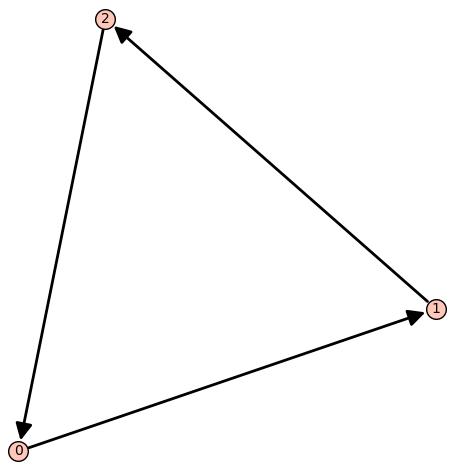
\includegraphics[width=0.3\textwidth]{3-vertices1.PNG}
%		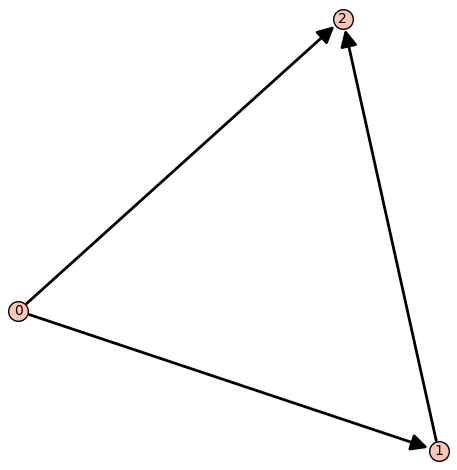
\includegraphics[width=0.3\textwidth]{3-vertices2.PNG}
%		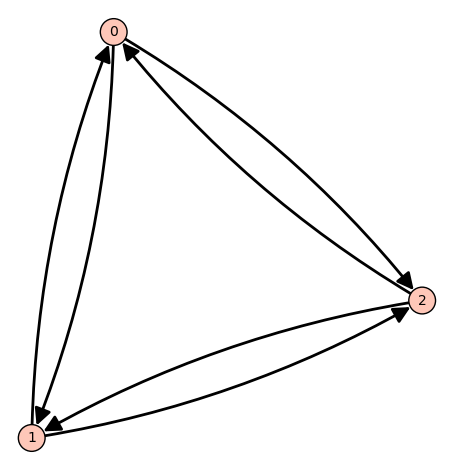
\includegraphics[width=0.3\textwidth]{3-vertices3.PNG}
%		\caption{Digrphs with Jacobians $0, \mathbb{Z}_2$, and $\mathbb{Z}_3$}
%		\end{figure}
			% cycle = Graph.cycle(3)
			% cycle.setEdgeState(0, 1, 2)
			% cycle.setEdgeState(1, 2, 2)
			% cycle.setEdgeState(2, 0, 2)
			% Trivial

			% cycle = Graph.cycle(3)
			% cycle.setEdgeState(0, 1, 1)
			% cycle.setEdgeState(1, 2, 2)
			% cycle.setEdgeState(2, 0, 2)
			% Z_2

			% cycle = Graph.cycle(3)
			% cycle.setEdgeState(0, 1, 0)
			% cycle.setEdgeState(1, 2, 0)
			% cycle.setEdgeState(2, 0, 0)
			% Z_3
%		\end{myeg}

%The number of paths in the cycle graph also plays a role in if it can represent all single term Jacobians up to $\mathbb{Z}_n$.
		

\begin{lem} \label{obj0}
Fix an orientation of $C_n$. If not every edge of $C_n$ (with a fixed orientation) is bidirectional, there is an orientation of $C_{n+1}$ such that $\Pic (C_n) \cong \Pic (C_{n+1})$. 
\end{lem}

\begin{proof}
Let $V(C_n)=\{v_1,\dots,v_n\}$ and $D_{C_n} = (d_{ij})$ be the diagonal matrix of $C_n$ (with a given orientation). Since not every edge is bidirectional, there exists $i$ such that $d_{ii} = 0$ or $1$. Without loss of generality, we may assume $i = n$ so that the adjacent vertices are $v_{n-1}$ and $v_1$. \\

\noindent \underline{Case 1:} Suppose that $d_{nn} = 0$. In this case, the Laplacian matrix of $C_n$ is the following. 
\begin{equation}
			L_{C_n} = 
			\begin{bmatrix}
				l + 1 & -l & 0 & \cdots & 0 & -1 \\
				\vdots & \vdots & \vdots & \cdots \\
				0 & \cdots & 0 & -k & k+1 & -1 \\
				0 & \cdots & 0 & 0 & 0 & 0 
			\end{bmatrix}
\end{equation}
			where $l, k \in \{ 0, 1 \}$. 
			We define $C_{n+1}$ extending $C_n$ as follows. 
			Add a vertex $v_{n+1}$ to $C_n$, replace the edge $e_{1\to n}$ by $e_{1 \to n+1}$, and add a new edge $e_{n \to n+1}$. 
			Pictorially, we have the following
			\begin{equation} \label{obj1}
				C_n: \left( \cdots \begin{tikzcd}[column sep=0.4cm]
					v_{n-1} \arrow[r] & v_n & v_1 \arrow[l] 
				\end{tikzcd} \cdots \right)
				\longrightarrow
				C_{n+1}: \left( \cdots \begin{tikzcd}[column sep=0.4cm]
					v_{n-1} \arrow[r] & v_n \arrow[r] & v_{n+1} &  v_1 \arrow[l] 
				\end{tikzcd} \cdots \right).
			\end{equation}
Now, one has the following equivalence of matrices.
			\begin{align*}
			L_{C_{n+1}} &= 
			\begin{bmatrix} 
				l + 1 & -l & 0 & \cdots & 0 & -1 \\
				\vdots & \vdots & \vdots & \cdots \\
				0 & \cdots & -k & k+1 & -1 &0 \\
				0 & \cdots & 0 & 0 & 1 & -1 \\
				0 & \cdots & 0 & 0 & 0 & 0 
			\end{bmatrix} 
			\stackrel{r_{1} \to r_1 - r_{n}}\longrightarrow
			\begin{bmatrix} 
				l + 1 & -l & 0 & \cdots & -1 & 0 \\
				\vdots & \vdots & \vdots & \cdots \\
				0 & \cdots & -k & k+1 & -1 &0 \\
				0 & \cdots & 0 & 0 & 1 & -1 \\
				0 & \cdots & 0 & 0 & 0 & 0 
			\end{bmatrix} \\
			&\stackrel{c_{n} \to c_{n} + c_{n+1}}\longrightarrow
			\begin{bmatrix} 
				l + 1 & -l & 0 & \cdots & -1 & 0 \\
				\vdots & \vdots & \vdots & \cdots \\
				0 & \cdots & -k & k+1 & -1 &0 \\
				0 & \cdots & 0 & 0 & 0 & -1 \\
				0 & \cdots & 0 & 0 & 0 & 0 
			\end{bmatrix}
			\longrightarrow
			\begin{bmatrix} 
				l + 1 & -l & 0 & \cdots & -1 & 0 \\
				\vdots & \vdots & \vdots & \cdots \\
				0 & \cdots & -k & k+1 & -1 &0 \\
				0 & \cdots & 0 & 0 & 0 & 0 \\
				0 & \cdots & 0 & 0 & 0 & 1 
			\end{bmatrix}\\
			&=
			\left[ \begin{array}{c|c}
				L_C & 0 \\
				\hline
				0 & 1
			\end{array} \right].
			\end{align*}
Now our claim follows from Remark \ref{remark: embedding}. \\

\noindent \underline{Case 2:} Now suppose $d_{nn} = 1$. Without loss of generality, we may assume the vertex $v_n$ has one outgoing edge to $v_1$. 
			There are two cases, depending on the existence of $e_{1\to n}$.
			The Laplacian of these two graphs are equivalent. 
\begin{equation}\label{equation: two equivalent matrices}
		L_{C_n} = \begin{bmatrix}
				l  & -l & 0 & \cdots & 0 & 0 \\
				\vdots & \vdots & \vdots & \cdots \\
				0 & \cdots & 0 & -k & k+1 & -1 \\
				-1 & \cdots & 0 & 0 & 0 & 1 
			\end{bmatrix}
			\stackrel{r_{1}\to r_1  - r_n}\longrightarrow
			\begin{bmatrix}
				l+1  & -l & 0 & \cdots & 0 & -1 \\
				\vdots & \vdots & \vdots & \cdots \\
				0 & \cdots & 0 & -k & k+1 & -1 \\
				-1 & \cdots & 0 & 0 & 0 & 1 
			\end{bmatrix},
\end{equation}
where $l, k \in \{ 0, 1 \}$. Therefore, we may assume that $L_{C_n}$ is the first matrix in \eqref{equation: two equivalent matrices}. We define $C_{n+1}$ extending $C_n$ as follows. Add a vertex $v_{n+1}$ to $C_n$, replace the edge $e_{n \to 1}$ by $e_{n+1 \to 1}$, and add a new edge $e_{n \to n+1}$. Pictorially, we have the following
\[
C_n: \left( \cdots \begin{tikzcd}[column sep=0.4cm]
					v_{n-1} \arrow[r] & v_n \arrow[r] & v_1 
				\end{tikzcd} \cdots \right)
				\longrightarrow
				C_{n+1}: \left( \cdots \begin{tikzcd}[column sep=0.4cm]
					v_{n-1} \arrow[r] & v_n \arrow[r] & v_{n+1} \arrow[r] & v_1 
				\end{tikzcd} \cdots \right).
			\]
	Then we have the following equivalence of matrices.
			\begin{align*}
			L_{C_{n+1}} &= 
			\begin{bmatrix} 
				l  & -l & 0 & \cdots & 0 & 0 & 0 \\
				\vdots & \vdots & \vdots & \cdots \\
				0 & \cdots & 0 & -k & k+1 & -1 & 0  \\
				0 & \cdots & 0 & 0 & 0 & 1 & -1 \\ 
				-1 & \cdots & 0 & 0 & 0 & 0 & 1 
			\end{bmatrix} \stackrel{r_{n+1}\leftrightarrow r_{n}}{\longrightarrow}
			\begin{bmatrix} 
				l  & -l & 0 & \cdots & 0 & 0 & 0 \\
				\vdots & \vdots & \vdots & \cdots \\
				0 & \cdots & 0 & -k & k+1 & -1 & 0  \\
				-1 & \cdots & 0 & 0 & 0 & 0 & 1 \\
				0 & \cdots & 0 & 0 & 0 & 1 & -1 
			\end{bmatrix} \\ 
			&\stackrel{r_{n} \to r_{n+1} + r_{n}}\longrightarrow 
			\begin{bmatrix} 
				l  & -l & 0 & \cdots & 0 & 0 & 0 \\
				\vdots & \vdots & \vdots & \cdots \\
				0 & \cdots & 0 & -k & k+1 & -1 & 0  \\
				-1 & \cdots & 0 & 0 & 0 & 1 & 0 \\ 
				0 & \cdots & 0 & 0 & 0 & 1 & -1 \\ 
			\end{bmatrix}
			\stackrel{c_{n} \to c_{n} - c_{n+1}}\longrightarrow 
			\begin{bmatrix} 
				l  & -l & 0 & \cdots & 0 & 0 & 0 \\
				\vdots & \vdots & \vdots & \cdots \\
				0 & \cdots & 0 & -k & k+1 & -1 & 0  \\
				-1 & \cdots & 0 & 0 & 0 & 1 & 0 \\ 
				0 & \cdots & 0 & 0 & 0 & 0 & -1 \\ 
			\end{bmatrix} \\
			&\longrightarrow 
			\left[ \begin{array}{c|c}
				L_C & 0 \\
				\hline
				0 & 1
			\end{array} \right].
			\end{align*}
Our claim follows from Remark \ref{remark: embedding}. 
		\end{proof}

\begin{lem} \label{obj4}
			For any $n \ge 4$ and any $m \in \{ n-1, n \}$, there exists an orientation of $C_n$ such that $\Jac (C_n) = \Z_m$. 
		\end{lem}

		\begin{proof}
If all edges of $C_n$ are bidirectional, then $\Pic (C_n) \cong \Z_n$. We claim that an orientation of $C_n$ such that 
			\[
			C_n: \left( \cdots \begin{tikzcd}[column sep=0.4cm]
				v_n \arrow[r] & v_1 & v_2 \arrow[l] & v_3 \arrow[l]
			\end{tikzcd} \cdots \right)
			\]
and all other edges are bidirectional has the Picard group $\mathbb{Z}_{n-1}$. In fact, we have the following equivalence of matrices:
			\begin{align*}
			L_{C_n} &= \begin{bmatrix}
				0 & 0 & 0 & 0 & 0 & 0 & 0 & 0   \\
				-1 & 1 & 0 & \cdots & 0 & 0 & 0 & 0  \\
				0 & -1 & 2 & -1 & \cdots & 0 & 0 & 0 \\
				0 & 0 & -1 & 2 & -1 & \cdots & 0 & 0  \\
				\vdots \\
				-1 & 0 & 0 & 0 & 0 & \cdots & -1 & 2 \\
			\end{bmatrix}
			\stackrel{r_{n} \to r_{n} - r_{2}}\longrightarrow
			\begin{bmatrix}
				0 & 0 & 0 & 0 & 0 & 0 & 0 & 0   \\
				-1 & 1 & 0 & \cdots & 0 & 0 & 0 & 0  \\
				0 & -1 & 2 & -1 & \cdots & 0 & 0 & 0 \\
				0 & 0 & -1 & 2 & -1 & \cdots & 0 & 0  \\
				\vdots \\
				0 & -1 & 0 & 0 & 0 & \cdots & -1 & 2 \\
			\end{bmatrix}\\
			&\stackrel{c_2 \to c_2+c_1}\longrightarrow
			\begin{bmatrix}
				0 & 0 & 0 & 0 & 0 & 0 & 0 & 0   \\
				-1 & 0 & 0 & \cdots & 0 & 0 & 0 & 0 \\
				0 & -1 & 2 & -1 & \cdots & 0 & 0 & 0 \\
				0 & 0 & -1 & 2 & -1 & \cdots & 0 & 0  \\
				\vdots \\
				0 & -1 & 0 & 0 & 0 & \cdots & -1 & 2 \\
			\end{bmatrix}
			\to
			\begin{bmatrix}
				1 & 0 & 0 & \cdots & 0 & 0 & 0 & 0 \\
				0 & 0 & 0 & 0 & 0 & 0 & 0 & 0   \\
				0 & -1 & 2 & -1 & \cdots & 0 & 0 & 0 \\
				0 & 0 & -1 & 2 & -1 & \cdots & 0 & 0  \\
				\vdots \\
				0 & -1 & 0 & 0 & 0 & \cdots & -1 & 2 \\
			\end{bmatrix}\\
			&\to\begin{bmatrix}
				1 & 0 & 0 & \cdots & 0 & 0 & 0 & 0 \\
				0 & 2 & -1 & 0 & 0 & 0 & 0 & -1   \\
				0 & -1 & 2 & -1 & \cdots & 0 & 0 & 0 \\
				0 & 0 & -1 & 2 & -1 & \cdots & 0 & 0  \\
				\vdots \\
				0 & -1 & 0 & 0 & 0 & \cdots & -1 & 2 \\
			\end{bmatrix} \tag{See the remark below for the last equivalance}
			\end{align*}
			Now the $(n-1) \times (n-1)$ bottom right submatrix is that of $C_{n-1}$ with all bidirecional edges and Remark \ref{remark: embedding} proves the claim.
		\end{proof}

		\begin{rmk} \label{obj2}
			For $n \ge 3$, the Lapacian of $C_n$ each of its eage is bidirecional, the Laplician of $C_n$ is of the form 
			$$
			L = 
			\begin{bmatrix}
				2 & -1 & 0 & 0 & 0 & 0 & -1   \\
				-1 & 2 & -1 & \cdots & 0 & 0 & 0 \\
				0 & -1 & 2 & -1 & \cdots & 0 & 0  \\
				\vdots \\
				-1 & 0 & 0 & 0 & \cdots & -1 & 2 \\
			\end{bmatrix}
			$$
			Since $[1 \cdots 1] L = 0$, 
			the first row is a $\Z$-linear combination of the next $(n-1)$ rows. 
			This justifies the last equivalence in the proof above.  
		\end{rmk}

		\begin{proof}[Proof of the Conjecture \ref{conjecture: single term}]
		We induct on the number of edges. The base case is when $n = 3$ which is Example \ref{example: example c3}. For $n > 3$, by Lemma \ref{obj4}, we have orientations of $C_n$ with $\Jac(C_n) = \mathbb{Z}_n$ and $\mathbb{Z}_{n-1}$. 
		Now the rest follows from Lemma \ref{obj0}. 
		%``This needs to be argued more carefully using maps between the set of the Jacobians for $C_n$ except for one.''
		\end{proof}
			
	

\subsection{Construction of cyclic Jacobians of $C_n$}
By a \textit{path} of $C_n$, we mean a connected subgraph of $C_n$ in which all arrows are oriented in a single direction or are bidirectional. In other words, a path is a subgraph of $C_n$ with one strong terminal component. 
				
In graphs with exactly two of these paths, a consistent pattern arises that allows for the rapid calculation of the Jacobian in only $O(n)$ time compared to the $O(n^4)$ time that calculating the Smith normal form takes. This pattern relies on calculating the number of bidirectional arrows between these two paths on one side. Our experimental computation suggests the following. 

		\begin{conj}\label{conjecture: two path}
			Let $C_n$ be a cycle graph with a fixed orientation. Then, we have $\Jac(G)=\mathbb{Z}_{x+2}$, where $x$ is the number of bidirectional edges clockwise of the counter-clockwise path and counter-clockwise of the clockwise path.
		\end{conj}
		%\begin{proof}
		%	We have proven this completely for cycle graphs up to $C_{80}$ when using two continuous paths without any bidirectional arrows separating them on the other size.  This has also held true for many other arbitrary orientations that still meet the two-path definition.	\end{proof}

		%This holds true for nearly every graph tested, with very few exceptions.

		\begin{lemma} \label{obj3}
			For $n \ge 2$, consider the following square matrix $M_n$
			\begin{equation}
				M_n = \begin{bmatrix}
					2 & -1 & 0 & 0& \cdots & \cdots & 0 \\
					-1 & 2 & -1& 0& \cdots &\cdots & 0 \\
					0 & -1 & 2 & -1 & 0& \cdots & 0 \\
					\vdots \\
					0 & 0 & \cdots& 0 & -1 & 2 & -1 \\
					0 & 0 &0 & \cdots & 0 &  -1 & 2 
					\end{bmatrix}.
			\end{equation}
			This is a matrix whose digonal entries are $2$ and sub-diagonals are $-1$. Then $\det (M_n) = n+1$. 
		\end{lemma}
		
		\begin{proof}
			We induct on $n$. 
			When $n=2$, a direct computation shows that $\det(M_2) = 3$. 
			Suppose the statement is true for all $k \le n-1$. 
			To compute $\det M_n$, 
			we use the Laplace expantion alone the first row.
			That is, $\det M_n = 2 \det (M_{n-1}) + \det(N)$, where $N$ is
			\begin{equation}
			N = \left[ \begin{array}{c|c c c c c  }
				-1 &  -1& 0 & \cdots & 0 \\
				\hline 
				0 &  &  M_{n-2}
			\end{array} \right].
			\end{equation}
			(Thus, $\det N = - \det (M_{n-2})$. \youngsu{to be removed})
			By induction, $\det M_n = 2 \det (M_{n-1}) - \det(M_{n-2}) = 2 (n-1+1) - (n-2+1) = 2n - n + 1 = n + 1.$
		\end{proof}
		
		\begin{rmk}
			Note that the $(n-1)$ by $(n-1)$ minor of $M_n$ after deleting the last row and last column is $(-1)^{n-1}$. 
			Hence the Smith normal form of $M_n$ is 
			\begin{equation}
			\left[ \begin{array}{c|c}
				I_{n-1} & 0 \\
				\hline 
				0 & n+1 
			\end{array} \right],
			\end{equation}
			where $I_{n-1}$ is the identity matrix of size $n-1$. 
		\end{rmk}
		
		\begin{lemma} Consider a directed cycle graph $C_n$ on $n$ vertices. 
		Assume that the vertex $v_1$ does not have any outgoing edge, and all other vertices have two outgoing edges. 
		Then $\Jac (C_n) = \mathbb{Z}_n$.
		\end{lemma}

		\begin{proof}
			The Laplacian of $C_n$ is 
			\begin{equation}
			\begin{bmatrix}
				0 & 0 & \cdots \\
				-1 & 2 & -1 & \cdots \\
				0 & -1 & 2 & -1 & \cdots \\
				\vdots \\
				0 &  \cdots& 0 & -1 & 2 & -1 \\
				-1 &  0 & \cdots & 0 &  -1 & 2 
			\end{bmatrix}. 
			\end{equation}
			By the same argument as in \Cref{obj2}, 
			\youngsu{we need to state \Cref{obj2} for the general case}
			This matrix is equivalent to 
			\begin{equation}
				\left[ \begin{array}{c|c}
					0 & 0 \\
					\hline 
					0 & M_{n-1}
				\end{array} \right],
			\end{equation}
			where $M_{n-1}$ is the matrix in \Cref{obj3}.
			Thus, by the remark above, $\Jac (C_n) = \mathbb{Z}_n$. 
			(One can also use the proof of \Cref{obj4} with \Cref{obj3}.)
		\end{proof}

		The general case follows from this lemma combined with the first and the second parts of the proof of \Cref{obj0} for $\mathbb{Z}_{n-1}$. (I believe Matt's observation about straightning intermediate birational edges corresponses to the reduction in the 2nd case of $d_{n,n}=1$.)

	%\subsection{Representing The Rank of the Picard Group for Cycle Graphs}
	%	The following example shows that the rank of $\Pic(C_n)$ (with an orientation) does not have to be $1$;	this directly follows from~\cite[Corollary 3.5]{wagner2000critical}.

%		\begin{myeg}
			%cycle = Graph.cycle(9)
			%cycle.setEdgeState(0, 1, 0)
			%cycle.setEdgeState(1, 2, 1)
			%cycle.setEdgeState(2, 3, 1)
			%cycle.setEdgeState(3, 4, 2)
			%cycle.setEdgeState(4, 5, 2)
			%cycle.setEdgeState(5, 6, 1)
			%cycle.setEdgeState(6, 7, 1)
			%cycle.setEdgeState(7, 8, 2)
			%cycle.setEdgeState(8, 0, 2)
			%Rank(Pic(G)) = 2: 2 terminal strong components
%		\end{myeg}

%		$\Pic(G)$ is often in the form $\mathbb{Z}_1 \times \dots \times \mathbb{Z}_n \times \mathbb{Z}^m$ where $m$ is the rank of the picard group.  A terminal strong component describes itself well.  It is a terminal component, meaning that its only connections are edges directed into it.  It is also strongly connected, meaning that every vertex in the component has at least one path to all other components.  For cycle graphs and trees, the number of these terminal strong components is exactly equal to $Rank(\Pic(G))$.

		%\begin{proof}
		%	The $Rank(\Pic(G))$ comes directly from the number of all zero rows of the Smith Normal Form of the laplacian of	$G$.  Terminal strong components are either already zero rows (in the case of a single sink) or there exists a series of row and column operations that, when preformed on the laplacian result in a row of allzeroes.
		%\end{proof}

%	\begin{lem}
%		Let $C_n$ be the cycle graph with $n$ vertices. Consider the equi-orientation of $C_n$. Then $\Pic(C_n)=\mathbb{Z}$.
	%\end{lem}
	%\begin{proof}
	%	In this case $C_n$ will always have a laplacian with a diagonal of $1$ and a diagonal of $-1$ above or below it depending on the orientation, with another $-1$ in the top right or bottom left corner where $V_0$ connects $V_{n-1}$.  Turing this laplacian into a smith normal form of all $1$s is as simple as cascading additions from the first row in a counter-clockwise case and the last row in the clockwise case. This will result in a diagonal of ones with the first or last column made up of mostly $-1$.  From here all that needs to be done is to eliminate these with the first or last row.  Since each equi-oriented $C_n$ will follow this pattern, this algorithm will prove $\Pic(C_n)=\mathbb{Z}$ for all $C_n$.
%	\end{proof}

%\section{Picard groups of oriented pseudotrees}

	\textcolor{red}{Jaiung: here we study how Picard groups change when we glue two directed graphs along one vertex or
		connect two graphs along one arrow. If we are lucky this should provide a way to compute Picard groups for
		pseudotrees by using the tree case and the cycle case in the previous sections.}

\section{Picard groups of oriented wheel graphs}

\textcolor{red}{Jaiung: the following conjecture should generalize the results in \cite{biggs1999chip}.}


	For wheel graphs, we looked for patterns that arose within the invariant factors of the Jacobian as a
	general formula was not immediately obvious.  For this strategy, we broke the edges of the wheel graph into their
	two most obvious groups, those belonging to the rim of the wheel and those of the spokes.  By orienting all the
	edges of either group the same way and trying all nine combinations, we noticed a well-defined pattern for each as
	the size of the wheel graph changed.  These patterns fell into four distinct groups.

		\begin{enumerate}
			\item When the spoke edges all pointed towards the axel and the rim was not bidirectional, or when
				the spoke edges were bidirectional, but the rim was not then a graph of size $n$ had a
				Jacobian of $\mathbb{Z}_{2^{(n-1)}-1}$.
			\item When the spoke edges all pointed away from the axel and the rim was not bidirectional,
				a graph of size $n$ had a Jacobian of $\mathbb{Z}_{n-1}$.
			\item When the spoke edges point away from the axel and the rim was bidirectional and a graph of size
				$n$ had a Jacobian of $\mathbb{Z}_{n-1} \times \mathbb{Z}_{n-1}$ when $n$ was even
				and $\mathbb{Z}_{\frac{n-1}{2}} \times \mathbb{Z}_{(n-1) \times 2}$ when $n$ was odd.
			\item When all edges were bidirectional or when the spoke direction was towards the axel and
				the rim was bidirectional, a graph of size $n$ had a Jacobian of
				$\mathbb{Z}_{\alpha\phi^{n}} \times \mathbb{Z}_{5\alpha\phi^{n}}$ when the size
				was odd where $\alpha \approxeq 0.27555$ and $\mathbb{Z}_{\beta\phi^{n}} \times \mathbb{Z}_{\beta\phi^{n}}$
				when the size was even where $\beta \approxeq 0.618035$. In both of these patterns,
				$\phi$ represents the golden ratio.
		\end{enumerate}

\begin{mydef}[{Wheel graph}]
By a wheel graph $W_n$, we mean a graph obtained by connecting a single universal vertex to all vertices of a cycle $C_{n-1}$. 
\end{mydef}

\begin{proposition}
Let $W_n$ be the wheel graph with bidirectional edges, and let $W_n'$ be the wheel graph such that the edges of the rim are bidirectional and all its spoke edges point to the axel. 
Then $L_{W_n}'$ and $L_{W_n}$ are row equivalent. In particular, one has $\Pic (W_n) \cong \Pic (W_n')$.
\end{proposition}

\begin{proof}
We use the labeling convention that $v_1$ is the axel and the vertices on the rim are $v_2, \dots, v_{n}$. One can directly see that the Laplacian matrices of $W_n$ and $W_n'$ are row equivalent. To be precise, from the Laplacian $L_{W_n'}$, one can obtain the Laplacian $L_{W_n}$ by subtracting all other rows from the first row by using the fact that the $\mathbf{1_n} \cdot L_{w_n} = 0$:
\[
	L_{W_n'} = \begin{bmatrix}
		0 & | & 0 & 0 & \cdots & \cdots & \cdots & \cdots & 0 \\
		\hline
		-1 & | & 3 & -1 & 0 & \cdots & \cdots & 0 & -1 \\
		-1 & | & - 1& 3 & -1 & \cdots & \cdots & 0 & 0 \\
		-1 & | & 0 & - 1& 3 & -1 & \cdots & 0 & 0 \\
		-1 & | & 0 & 0 & - 1& 3 & -1 & \cdots & 0 \\
		-1 & | & \vdots & \vdots \\
		-1 & | & 0 & 0 & 0 & \cdots & -1& 3 & -1 \\
		-1 & | & -1 & 0 & 0 & \cdots& 0 & -1 & 3 
	\end{bmatrix}
\]
\[
L_{W_n} = \begin{bmatrix}
		n-1 & | & -1 & -1 & \cdots & \cdots & \cdots & \cdots & -1 \\
		\hline
		-1 & | & 3 & -1 & 0 & \cdots & \cdots & 0 & -1 \\
		-1 & | & - 1& 3 & -1 & \cdots & \cdots & 0 & 0 \\
		-1 & | & 0 & - 1& 3 & -1 & \cdots & 0 & 0 \\
		-1 & | & 0 & 0 & - 1& 3 & -1 & \cdots & 0 \\
		-1 & | & \vdots & \vdots \\
		-1 & | & 0 & 0 & 0 & \cdots & -1& 3 & -1 \\
		-1 & | & -1 & 0 & 0 & \cdots& 0 & -1 & 3 
	\end{bmatrix}
\]

%where the top row of $L_{w_n}$ is the negative of the sum of the remaining rows. (Use the fact that the $\mathbf{1_n} \cdot L_{w_n} = 0$. )
% Recall the submatrix after deleting the first row and column is of the form 
% $L_{C_{n-1}} + I_n$, where $C_{n-1}$ is the bidirectional cyclec graph on $n-1$ vertices. 
% The sum of the rows of $L_{C_{n-1}} = 0$. 
\end{proof}

\youngsu{This approach probably works for complete graphs where all edges are bidirectional except for one vertex.}

\begin{proposition}
Let $W_n$ be the wheel graph where the edges of the rim are bidirectional and all its spoke edges point away from the axel. Then the Smith normal form of the Laplacian of $W_n$ is of the following form 
\begin{equation*}
\left[
\begin{array}{c|ccc}	
I_{n-3} & 0 & 0 & 0 \\
\hline
0 & a & 0 & 0 \\
0 & 0 & b & 0 \\
0 & 0 & 0 & 0 
\end{array}
\right], \quad \textrm{ where } (a,b) = \begin{cases}
	(n-1,n-1) & \text{if}~ n ~\text{is even}; \\
	(\frac{n-1}2, 2(n-1)) & \text{if}~ n ~\text{is odd}
\end{cases}
\end{equation*}
\end{proposition}
\begin{proof}
We use the labeling convention that $v_1$ is the axel and the vertices on the rim are $v_2, \dots, v_{n}$.  
%Note that the rim of $W_n$ in this case is an undirected (bidirectional) cycle graph $C_{n-1}$ whose Laplacian has the following Smith normal form.
%\begin{equation*}
%\left[
%	\begin{array}{c|ccc}	
%	I_{n-3} & 0 & 0 \\
%	\hline
%	0 & n-1 & 0 &\\
%	0 & 0 & 0 &
%	\end{array}
%\right]. 
%\end{equation*}
%Since $C_{n-1}$ is a subgraph of $W_n$, 
Let $L_{W_n}$ be the Laplacian matrix of $W_n$. It is clear that $\det(L_{W_n})=0$. Hence, from Theorem \ref{theorem: gcd theorem}, it suffices to show that 
\begin{equation*}
I_{n-1}(L_{W_n}) = \langle (n-1)^2 \rangle~\text{and}~ I_{n-2}(L_{W_n}) = \begin{cases}
\langle n-1 \rangle & \text{if}~ n ~\text{is even} \\
\langle (n-1)/2\rangle & \text{if}~ n ~\text{is odd}.
\end{cases}
\end{equation*}
We reduce its Laplacian matrix $L_{W_n}$ as follows:
\[
L_{W_n}=\scalemath{0.85}{\begin{bmatrix}
	n-1 & | & -1 & -1 & \cdots & \cdots & \cdots & \cdots & -1 \\
	\hline
	0 & | & 2 & -1 & 0 & \cdots & \cdots & 0 & -1 \\
	0 & | & - 1& 2 & -1 & \cdots & \cdots & 0 & 0 \\
	0 & | & 0 & - 1& 2 & -1 & \cdots & 0 & 0 \\
	0 & | & 0 & 0 & - 1& 2 & -1 & \cdots & 0 \\
	0 & | & \vdots & \vdots \\
	0 & | & 0 & 0 & 0 & \cdots & -1& 2 & -1 \\
	0 & | & -1 & 0 & 0 & \cdots& 0 & -1 & 2 
\end{bmatrix} 
\stackrel{c_1 \to c_1 + \cdots + c_n}\longrightarrow \begin{bmatrix}
	0 & | & -1 & -1 & \cdots & \cdots & \cdots & \cdots & -1 \\
	\hline
	0 & | & 2 & -1 & 0 & \cdots & \cdots & 0 & -1 \\
	0 & | & - 1& 2 & -1 & \cdots & \cdots & 0 & 0 \\
	0 & | & 0 & - 1& 2 & -1 & \cdots & 0 & 0 \\
	0 & | & 0 & 0 & - 1& 2 & -1 & \cdots & 0 \\
	0 & | & \vdots & \vdots \\
	0 & | & 0 & 0 & 0 & \cdots & -1& 2 & -1 \\
	0 & | & -1 & 0 & 0 & \cdots& 0 & -1 & 2 
\end{bmatrix} }
\]
\vspace{0.2cm}
\[
\scalemath{0.85}{ \stackrel{r_n \to r_2 + \cdots + r_{n}}\longrightarrow
\begin{bmatrix}
	0 & | & 1 & 1 & \cdots & \cdots & \cdots & \cdots & 1 \\
	\hline
	0 & | & 2 & -1 & 0 & \cdots & \cdots & 0 & -1 \\
	0 & | & - 1& 2 & -1 & \cdots & \cdots & 0 & 0 \\
	0 & | & 0 & - 1& 2 & -1 & \cdots & 0 & 0 \\
	0 & | & 0 & 0 & - 1& 2 & -1 & \cdots & 0 \\
	0 & | & \vdots & \vdots \\
	0 & | & 0 & 0 & 0 & \cdots & -1& 2 & -1 \\
	0 & | & 0 & 0 & 0 & \cdots& 0 & 0 & 0
\end{bmatrix}
\stackrel{c_n \to c_2 + \cdots + c_{n}}\longrightarrow
\begin{bmatrix}
	0 & | & 1 & 1 & \cdots & \cdots & \cdots & 1 & n-1 \\
	\hline
	0 & | & 2 & -1 & 0 & \cdots & \cdots & 0 & 0 \\
	0 & | & - 1& 2 & -1 & \cdots & \cdots & 0 & 0 \\
	0 & | & 0 & - 1& 2 & -1 & \cdots & 0 & 0 \\
	0 & | & 0 & 0 & - 1& 2 & -1 & \cdots & 0 \\
	0 & | & \vdots & \vdots \\
	0 & | & 0 & 0 & 0 & \cdots & -1& 2 & 0 \\
	0 & | & 0 & 0 & 0 & \cdots& 0 & 0 & 0
\end{bmatrix} }
\]
%\begin{align}
%L_{W_n} = \begin{bmatrix}
%n-1 & | & 1 & 1 & \cdots & \cdots & \cdots & \cdots & 1 \\
%\hline
%0 & | & 2 & -1 & 0 & \cdots & \cdots & 0 & -1 \\
%0 & | & - 1& 2 & -1 & \cdots & \cdots & 0 & 0 \\
%0 & | & 0 & - 1& 2 & -1 & \cdots & 0 & 0 \\
%0 & | & 0 & 0 & - 1& 2 & -1 & \cdots & 0 \\
%0 & | & \vdots & \vdots \\
%0 & | & 0 & 0 & 0 & \cdots & -1& 2 & -1 \\
%0 & | & -1 & 0 & 0 & \cdots& 0 & -1 & 2 
%\end{bmatrix}
%\stackrel{C_1 \to C_1 + \cdots + C_n}\sim
%\begin{bmatrix}
%0 & | & 1 & 1 & \cdots & \cdots & \cdots & \cdots & 1 \\
%\hline
%0 & | & 2 & -1 & 0 & \cdots & \cdots & 0 & -1 \\
%0 & | & - 1& 2 & -1 & \cdots & \cdots & 0 & 0 \\
%0 & | & 0 & - 1& 2 & -1 & \cdots & 0 & 0 \\
%0 & | & 0 & 0 & - 1& 2 & -1 & \cdots & 0 \\
%0 & | & \vdots & \vdots \\
%0 & | & 0 & 0 & 0 & \cdots & -1& 2 & -1 \\
%0 & | & -1 & 0 & 0 & \cdots& 0 & -1 & 2 
%\end{bmatrix}\\
%%%%
%\stackrel{R_n \to R_2 + \cdots + R_{n}}\sim
%\begin{bmatrix}
%0 & | & 1 & 1 & \cdots & \cdots & \cdots & \cdots & 1 \\
%\hline
%0 & | & 2 & -1 & 0 & \cdots & \cdots & 0 & -1 \\
%0 & | & - 1& 2 & -1 & \cdots & \cdots & 0 & 0 \\
%0 & | & 0 & - 1& 2 & -1 & \cdots & 0 & 0 \\
%0 & | & 0 & 0 & - 1& 2 & -1 & \cdots & 0 \\
%0 & | & \vdots & \vdots \\
%0 & | & 0 & 0 & 0 & \cdots & -1& 2 & -1 \\
%0 & | & 0 & 0 & 0 & \cdots& 0 & 0 & 0
%\end{bmatrix}
%%%%
%\stackrel{C_n \to C_2 + \cdots + C_{n}}\sim
%\begin{bmatrix}
%0 & | & 1 & 1 & \cdots & \cdots & \cdots & 1 & n-1 \\
%\hline
%0 & | & 2 & -1 & 0 & \cdots & \cdots & 0 & 0 \\
%0 & | & - 1& 2 & -1 & \cdots & \cdots & 0 & 0 \\
%0 & | & 0 & - 1& 2 & -1 & \cdots & 0 & 0 \\
%0 & | & 0 & 0 & - 1& 2 & -1 & \cdots & 0 \\
%0 & | & \vdots & \vdots \\
%0 & | & 0 & 0 & 0 & \cdots & -1& 2 & 0 \\
%0 & | & 0 & 0 & 0 & \cdots& 0 & 0 & 0
%\end{bmatrix}.
%\end{align}
\vspace{0.2cm}

\noindent Thus, to compute the Smith normal form of $L_{W_n}$, it suffices to find the Smith normal form of the following matrix.
\begin{equation*}
N = \left[
	\begin{array}{c|c}
	\mathbf{1}_{n-2} & n-1 \\
	\hline
	M_{n-2} & \mathbf{0}_{n-1}
	\end{array}
\right],
\end{equation*}
where $M_{n-2}$ is the matrix in \Cref{obj3}. 
Note that $\det(M_{n-2}) = n-1$ and this shows that $I_{n-1}(L_{W_n}) = I_{n-1}(N) = \angles{\det(N)}=\angles{(n-1)^2}$.

To compute the $(n-2)$ minors, first note that if the last column is a part of a minor, then it is divisible by $n-1$. 
Since $\det(M_{n-2}) = n-1 \in I_{n-2}(N)$, we only need to consider the $n-2$ minors of the first $n-2$ columns of $N$. 

In other words, $I_{n-2}(L_{W_n})$ is generated by $n-1$ 
and the $(n-2)$-determinents of the matrix which is obtained from $M_{n-2}$ by replacing the $i^{\textrm{th}}$ row by $\mathbf{1}_{n-2}$.

Note that $M_{n-2}$ is symmetric. 
By Cramer's rule, these $(n-2)$-minors are the entries of the solution matrix $\mathbf{x}$ of the matrix equation
\begin{equation*}
M_{n-2} \mathbf{x} 
= \det(M_{n-2}) \cdot \mathbf{1}_{n-2}^T
\end{equation*}
up to sign.
This is done in the following lemma, and it completes the proof.
\end{proof}

\begin{lemma}\label{M_nCremer}
% Let $M_n$ as in \Cref{obj3}. That is
% \begin{equation*}
% 	M_n = \begin{bmatrix}
% 		2 & -1 & 0 & 0& \cdots & \cdots & 0 \\
% 		-1 & 2 & -1& 0& \cdots &\cdots & 0 \\
% 		0 & -1 & 2 & -1 & 0& \cdots & 0 \\
% 		\vdots \\
% 		0 & 0 & \cdots& 0 & -1 & 2 & -1 \\
% 		0 & 0 &0 & \cdots & 0 &  -1 & 2 
% 		\end{bmatrix}.
% \end{equation*}
Consider the matrix equation 
\begin{equation*}
M_n \mathbf{x} 
= \det(M_n) \mathbf{1_n}^T
= (n+1) \mathbf{1_n}^T,
\end{equation*}
where $M_n$ is as in $\Cref{obj3}$. 
Let $x_k$ denote the $k^{\textrm{th}}$ entry of $\mathbf{x}$. Then $x_k = a k^2 + b k$, where
\[
a = -\frac{(n+1)}{2}, \quad b = \frac{(n+1)^2}{2}.
\]
Furthermore, $\gcd(x_1,\dots, x_n)$ is $n+1$ if $n$ is even and $(n+1)/2$ if $n$ is odd. 
\end{lemma}

\begin{proof}
% Note that since $M_n$ is invertible over $\mathbb{Q}$, the solution exists and unique over $\mathbb{Q}$.
% Since $\mathbb{Z} \subset \mathbb{Q}$, once we find a solution, it suffices to show that the entries of $\mathbf{x}$ are integers. 
Note that $\det (M_n) = n+1$ (\Cref{obj3}). 
Consider a sequence $f(k)=f_k  = ak^2 + bk$. 
For any $k$, we have
\[
-f_{k-1} + 2f_k - f_{k+1} = -2a.
\]
First, we set $a = -(n+1)/2$. 
In addition, the equations $2x_1 - x_2 = n+1$ and $-x_{n-1} + 2x_n = n+1$ are equivalent to the conditions $f_0 = f_{n+1} = 0$. 
These conditions imply $b = (n+1)^2/2$ since $0, -b/a$ are the roots of $f(k)$. 

We compute the gcd of $f_1,\dots, f_n$. 
First, we claim that $\gcd(f_1,\dots, f_n) = \gcd(f_1, n+1)$. 
Since $\gcd(f_1,\dots, f_n)$ divides $2f_1-f_2 = n+1$, 
it suffices to show that $\gcd(f_1, n+1)$ divides $f_2,\dots, f_n$. 
This folows by induction since for $k = 2, \dots, n$, 
$f_k = 2 f_{k-1} - f_{k-2} - (n+1)$.
Here we use the fact that $f_0 = 0$. 
Since $f_1 =  -(n+1)/2 + (n+1)^2/2 = \frac{n(n+1)}2$ is an integer, the expressions $f_k = -2 f_{k-1} + f_{k-2}$ also proves that $f_1, \dots, f_n$ are integers. 

Finally, we show that $\gcd(f_1, n+1)$ is $n+1$ when $n$ is even and $(n+1)/2$ when $n$ is odd. 
Recall that $f_1 = \frac{n(n+1)}2$.
If $n$ is even, then $n+1$ divides $f_1$. 
Thus, $\gcd(f_1, n+1) = n+1$. 
If $n$ is odd, then 
\[
\gcd(f_1, n+1) = \gcd(\frac{n+1}2 \cdot n, n+1) = \gcd(\frac{n+1}2, n+1) = \frac{n+1}2.
\] 
The $2^\textrm{nd}$ last equality follows from the fact that $\frac{n+1}2$ is an integer and for integers $a,b,c$, $\gcd(ab,c) = \gcd(a,c)$ if $b,c$ are relatively prime. 

Thus $\mathbf{x} = \begin{bmatrix} f_1 & \cdots & f_n \end{bmatrix}^T$ is a solution having the asserted gcd. 
This completes the proof. 
\end{proof}



\section{Picard groups of oriented multipartite graphs}
\textcolor{red}{Jaiung: this paper \cite{jacobson2003critical} could be relevant here.}
	For our purposes, a multipartite graph is a graph whos vertices can be partitioned between several independent
	groups, arranged in a linear order.  Vertices have no connections to members of their own group, but are strongly
	connected to all vertices of their two adjacent groups.

	The structure of the graphs that we investigate are intentionally designed to resemble artificial neural networks.
	To further facilitate this comparison, we direct all edges \textit{forward} such that, after numbering the groupings
	of these vertices in some order, edges always point towards the next highest numbered grouping.

	We were able to find notable patterns in both a \textit{Perceptron} style model with two layers and a
	\textit{Hidden Layer} model with three layers.

	\subsection{Picard groups for two layers}
		For two layers in the form of $f \rightarrow s$ where $f$ and $s$ are the number of nodes in the first and
		second layers, respectively, $\Pic(G) = \mathbb{Z}_{s}^{f-1} \times \mathbb{Z}^s$.

	\subsection{Picard groups for three layers}
		For three layers in the form of $f \rightarrow s \rightarrow t$ where $f$, $s$, and $t$ are the number of nodes
		in the first, second, and third layers, respectively the Picard group is significantly more complex.

		\begin{enumerate}
			\item When ($s$ is odd, $s$ is not a factor of $t$ and $f <= s$) or
					($t$ is odd, $s$ is even, and $f <= s$) or
				$\Pic(G) = Z_{t}^{s-f-1} \times Z_{s \times t}^{f} \times Z^t$

			\item When ($s$ is odd, $s$ is not a factor of $t$ and $f > s$) or
					($t$ is odd, $s$ is even and $f > s$),
				$\Pic(G) = Z_{s}^{f-s+1} \times Z_{s \times t}^{s-1} \times Z^t$

			\item When ($s$ is odd and $s$ is a factor of $t$) or ($t$ is even, $s$ is even, and $s$ is a factor of $t$),
				$\Pic(G) = Z_{s}^{f-1} \times Z_{t} \times Z_{s \times t} \times Z^t$

			\item When ($t$ is even, $s$ is even, and $s$ is a not factor of $t$),
				$\Pic(G) = Z_{2}^{f-1} \times Z_{t}^{s-f-1} \times Z_{s \times t/2}^{f-1} \times Z_{s \times t} \times Z^t$
		\end{enumerate}

\section{Experimental Results}

\section{Conjectures and Future directions}

	\begin{conj}
		For any cycle graph $C_n$, the orientation with no paths always has a Jacobian of $\mathbb{Z}_n$.
		Either of the single path orientations have a trivial Jacobian.
		The set of all orientations with two paths always contains all single invariant factors
		$\mathbb{Z}_2\dots\mathbb{Z}_n$.  For all graphs at least up to $C_{10}$ and likely well beyond that
		point, the sets that contain all other paths do not contain all of the single invariant factors. \textcolor{red}{Jaiung: I think this should not be difficult....}
	\end{conj}

It should be noted that for four paths and upward, the sets that contain these paths often also contain
Jacobians of $\mathbb{Z}_3$ and $\mathbb{Z}_4$.  The number of each of these increases with the size of the
graph, so it is possible that these sets will contain all of the single invariant factors for very
large cycle graphs.

\subsection{Experimental Results of Wheel Graphs}

	\begin{conj}
		For wheel graphs of size $n$, when ($n$ is even or $n-1 | 4$) and all spokes point outward, the Picard groups appear to follow
		$\mathbb{Z}_{(n-1) \times a} \times \mathbb{Z}$ when the Picard group of the cycle graph of the same orientation as the rim
		and size $n-1$ is $\mathbb{Z}_a \times \mathbb{Z}$.

		When $n-1 | 2$, the Picard groups appear to follow $\mathbb{Z}_2 \times \mathbb{Z}_{(n-1)/2 \times a} \times \mathbb{Z}$.
	\end{conj}

	This appears to hold for any arbitrary rim orientation so long as the spokes all point outward.

	For example, for a cycle graph $C$ of size $9$ and an orientation such that $\Pic(C) = \mathbb{7} \times \mathbb{Z}$,
	the wheel graph of size $10$ with that same orientation in its rim has a Picard group of $\mathbb{63} \times \mathbb{Z}$

\bibliography{Jacobian}
\bibliographystyle{alpha}

\end{document}
